\documentclass[journal,12pt,twocolumn]{IEEEtran}
%
\usepackage{setspace}
\usepackage{gensymb}
\usepackage{siunitx}
\usepackage{tkz-euclide} 
\usepackage{textcomp}
\usepackage{standalone}
\usetikzlibrary{calc}
\newcommand\hmmax{0}
\newcommand\bmmax{0}

%\doublespacing
\singlespacing

%\usepackage{graphicx}
%\usepackage{amssymb}
%\usepackage{relsize}
\usepackage[cmex10]{amsmath}
%\usepackage{amsthm}
%\interdisplaylinepenalty=2500
%\savesymbol{iint}
%\usepackage{txfonts}
%\restoresymbol{TXF}{iint}
%\usepackage{wasysym}
\usepackage{amsthm}
%\usepackage{iithtlc}
\usepackage{mathrsfs}
\usepackage{txfonts}
\usepackage{stfloats}
\usepackage{bm}
\usepackage{cite}
\usepackage{cases}
\usepackage{subfig}
%\usepackage{xtab}
\usepackage{longtable}
\usepackage{multirow}
%\usepackage{algorithm}
%\usepackage{algpseudocode}
\usepackage{enumitem}
\usepackage{mathtools}
\usepackage{steinmetz}
\usepackage{tikz}
\usepackage{circuitikz}
\usepackage{verbatim}
\usepackage{tfrupee}
\usepackage[breaklinks=true]{hyperref}
%\usepackage{stmaryrd}
\usepackage{tkz-euclide} % loads  TikZ and tkz-base
%\usetkzobj{all}
\usetikzlibrary{calc,math}
\usepackage{listings}
    \usepackage{color}                                            %%
    \usepackage{array}                                            %%
    \usepackage{longtable}                                        %%
    \usepackage{calc}                                             %%
    \usepackage{multirow}                                         %%
    \usepackage{hhline}                                           %%
    \usepackage{ifthen}                                           %%
  %optionally (for landscape tables embedded in another document): %%
    \usepackage{lscape}     
\usepackage{multicol}
\usepackage{chngcntr}
\usepackage{amsmath}
\usepackage{cleveref}
\usepackage{amsmath}
%\usepackage{enumerate}

%\usepackage{wasysym}
%\newcounter{MYtempeqncnt}
\DeclareMathOperator*{\Res}{Res}
%\renewcommand{\baselinestretch}{2}
\renewcommand\thesection{\arabic{section}}
\renewcommand\thesubsection{\thesection.\arabic{subsection}}
\renewcommand\thesubsubsection{\thesubsection.\arabic{subsubsection}}

\renewcommand\thesectiondis{\arabic{section}}
\renewcommand\thesubsectiondis{\thesectiondis.\arabic{subsection}}
\renewcommand\thesubsubsectiondis{\thesubsectiondis.\arabic{subsubsection}}

% correct bad hyphenation here
\hyphenation{op-tical net-works semi-conduc-tor}
\def\inputGnumericTable{}                                 %%

\lstset{
%language=C,
frame=single, 
breaklines=true,
columns=fullflexible
}
%\lstset{
%language=tex,
%frame=single, 
%breaklines=true
%}
\usepackage{graphicx}
\usepackage{pgfplots}

\begin{document}


\newtheorem{theorem}{Theorem}[section]
\newtheorem{problem}{Problem}
\newtheorem{proposition}{Proposition}[section]
\newtheorem{lemma}{Lemma}[section]
\newtheorem{corollary}[theorem]{Corollary}
\newtheorem{example}{Example}[section]
\newtheorem{definition}[problem]{Definition}
%\newtheorem{thm}{Theorem}[section] 
%\newtheorem{defn}[thm]{Definition}
%\newtheorem{algorithm}{Algorithm}[section]
%\newtheorem{cor}{Corollary}
\newcommand{\BEQA}{\begin{eqnarray}}
\newcommand{\EEQA}{\end{eqnarray}}
\newcommand{\define}{\stackrel{\triangle}{=}}
\bibliographystyle{IEEEtran}
%\bibliographystyle{ieeetr}
\providecommand{\mbf}{\mathbf}
\providecommand{\abs}[1]{\ensuremath{\left\vert#1\right\vert}}
\providecommand{\norm}[1]{\ensuremath{\left\lVert#1\right\rVert}}
\providecommand{\mean}[1]{\ensuremath{E\left[ #1 \right]}}
\providecommand{\pr}[1]{\ensuremath{\Pr\left(#1\right)}}
\providecommand{\qfunc}[1]{\ensuremath{Q\left(#1\right)}}
\providecommand{\sbrak}[1]{\ensuremath{{}\left[#1\right]}}
\providecommand{\lsbrak}[1]{\ensuremath{{}\left[#1\right.}}
\providecommand{\rsbrak}[1]{\ensuremath{{}\left.#1\right]}}
\providecommand{\brak}[1]{\ensuremath{\left(#1\right)}}
\providecommand{\lbrak}[1]{\ensuremath{\left(#1\right.}}
\providecommand{\rbrak}[1]{\ensuremath{\left.#1\right)}}
\providecommand{\cbrak}[1]{\ensuremath{\left\{#1\right\}}}
\providecommand{\lcbrak}[1]{\ensuremath{\left\{#1\right.}}
\providecommand{\rcbrak}[1]{\ensuremath{\left.#1\right\}}}
\theoremstyle{remark}
\newtheorem{rem}{Remark}
\newcommand{\sgn}{\mathop{\mathrm{sgn}}}
\providecommand{\res}[1]{\Res\displaylimits_{#1}} 
%\providecommand{\norm}[1]{\lVert#1\rVert}
\providecommand{\mtx}[1]{\mathbf{#1}}
\providecommand{\fourier}{\overset{\mathcal{F}}{ \rightleftharpoons}}
%\providecommand{\hilbert}{\overset{\mathcal{H}}{ \rightleftharpoons}}
\providecommand{\system}{\overset{\mathcal{H}}{ \longleftrightarrow}}
	%\newcommand{\solution}[2]{\textbf{Solution:}{#1}}
\newcommand{\solution}{\noindent \textbf{Solution: }}
\newcommand{\cosec}{\,\text{cosec}\,}
\providecommand{\dec}[2]{\ensuremath{\overset{#1}{\underset{#2}{\gtrless}}}}
\newcommand{\myvec}[1]{\ensuremath{\begin{pmatrix}#1\end{pmatrix}}}
\newcommand{\mydet}[1]{\ensuremath{\begin{vmatrix}#1\end{vmatrix}}}
%\numberwithin{equation}{section}
\numberwithin{equation}{subsection}
%\numberwithin{problem}{section}
%\numberwithin{definition}{section}
\makeatletter
\@addtoreset{figure}{problem}
\makeatother
\let\StandardTheFigure\thefigure
\let\vec\mathbf
%\renewcommand{\thefigure}{\theproblem.\arabic{figure}}
\renewcommand{\thefigure}{\theproblem}
%\setlist[enumerate,1]{before=\renewcommand\theequation{\theenumi.\arabic{equation}}
%\counterwithin{equation}{enumi}
%\renewcommand{\theequation}{\arabic{subsection}.\arabic{equation}}
\def\putbox#1#2#3{\makebox[0in][l]{\makebox[#1][l]{}\raisebox{\baselineskip}[0in][0in]{\raisebox{#2}[0in][0in]{#3}}}}
     \def\rightbox#1{\makebox[0in][r]{#1}}
     \def\centbox#1{\makebox[0in]{#1}}
     \def\topbox#1{\raisebox{-\baselineskip}[0in][0in]{#1}}
\vspace{3cm}
\title{Assignment-6\\}
\author{Ayush Kumar}
\maketitle
\newpage
%\tableofcontents
\bigskip
\renewcommand{\thefigure}{\theenumi}
\renewcommand{\thetable}{\theenumi}
\begin{abstract}
This document contains solution of Problem Lonet\brak{314,5}
\end{abstract}
Download latex-tikz codes from 
%
\begin{lstlisting}
https://github.com/ayushkesh/Matrix-Theory-EE5609/tree/master/A6
\end{lstlisting}
\section{\textbf{Question}}
What conics do the given equations represent?\\
$6x^2-5xy-6y^2+14x+5y+4=0$
%\begin{align}
    %ax^2+2bxy+cy^2+2dx+2ey+f&=0\label{eqmain}
    %\intertext{the above equation \eqref{eqmain} can be expressed as}
    %\vec{V}=\vec{V}^T&=\myvec{a & b \\ b & c}\label{eq2}\\
    %\vec{u}&=\myvec{d \\ e}\label{eq3}
%\end{align}
%\begin{align}
%    \intertext{where}
%    \begin{array}{|cc|}
%\vec{V} & \vec{u}\\\vec{u}^T & f
%\end{array}&=0\label{eqcheck}
%\end{align}
\section{Solution}
%Given,
%\begin{align}
%\end{align}
The above equation can be expressed in the form 
\begin{align}
\vec{x}^T\vec{V}\vec{x}+2\vec{u}^T\vec{x}+f&=0\label{2.2} \label{eq1}
\intertext{Comparing equation we get}
    \vec{V}=\vec{V}^T&=\myvec{6 & \frac{-5}{2}\\\frac{-5}{2} &-6}\label{eqv}\\
    \vec{u}&=\myvec{7 \\ \frac{5}{2}}\label{equ}\\
    f&=4\label{eqfv}
\end{align}    
The above equation \eqref{eq1} represents a pair of straight lines if
\begin{align}
    \begin{array}{|cc|}
\vec{V} & \vec{u}\\\vec{u}^T & f
\end{array}&=0\label{eqcheck}
\end{align}
Verify the given equation as if it is pair of straight lines
\begin{align}
\Delta&=\begin{array}{|ccc|}
6 &\frac{-5}{2}& 7\\\frac{-5}{2} & -6 & \frac{5}{2}\\ 7 & \frac{5}{2} & 4
\end{array}\\
\implies \ 6\mydet{-6 & \frac{5}{2} \\ \frac{5}{2} & 4} 
		& -\frac{-5}{2}\mydet{-\frac{5}{2} & \frac{5}{2} \\ 7 & 4}
		+7\mydet{-\frac{5}{2} & -6 \\ 7 & \frac{5}{2}} = 0 \label{eq10}\\
\implies \Delta&=0
\end{align}
Since equation \eqref{eqcheck} is satisfied, we could say that the given equation represents two straight lines
\begin{align}
    \Delta_{V} &= \begin{array}{|cc|}
6 &\frac{-5}{2}\\\frac{-5}{2} & -6
\end{array}<0
\end{align}
Let the equations of lines be,
\begin{align}
	\brak{\vec{n_1}^T \vec{x} - c_1}\brak{\vec{n_1}^T \vec{x} - c_1} =
        \vec{x}^{T}\vec{Vx} + 2\vec{u}^{T}\vec{x} + f=0\label{eq:eql03}
\end{align}
\begin{align}
\brak{\vec{n_1}^T\vec{x}-c_1}\brak{\vec{n_2}^T\vec{x}-c_2}
&=\vec{x}^T\myvec{6 & \frac{-5}{2} \\\frac{-5}{2} & -6}\vec{x}\notag\\
+2\myvec{7 & \frac{5}{2}}\vec{x}+4\label{equate}\\
    \vec{n_1}*\vec{n_2} = \myvec{a\\2b\\c} &= \myvec{6\\-5\\-6}\label{conv}\\
    c_2\vec{n_1}+c_1\vec{n_2}&=-2\myvec{7\\\frac{5}{2}}\label{eqc1c2}\\
    c_1c_2&=4
\end{align}
The slopes of the lines are given by the roots of the polynomial 
\begin{align}
    &cm^2+2bm+a=0\label{e}\\
    \implies m_i&=\frac{-b\pm{\sqrt{-\Delta_{V}}}}{c}\\
    \vec{n_i}&=k\myvec{-m_i\\1}
\end{align}
Substituting the given data in above equations \eqref{e} we get,
\begin{align}
    &-6m^2-5m+6=0\\
    &\implies m_i=\frac{\frac{-5}{2}\pm{\sqrt{-(\frac{-169}{4})}}}{-6}\label{m}
\intertext{Solving equation \eqref{m} we get,}
    m_1&=-\frac{3}{2},  m_2=\frac{2}{3}\\
   % \vec{m_1}=\myvec{-2\\3}, \vec{m_2}=\myvec{3\\ 2}\\
   &= \vec{n_1}=\myvec{-3\\ -2}, \vec{n_2}=\myvec{-2\\3} \label{eq:normal1}
\intertext{We know that,}
\vec{n_1}\ast \vec{n_2} = \myvec{a\\2b\\c} \label{eq:conv1}
\end{align}
Verification using Toeplitz matrix, From equation \eqref{eq:normal1}
\begin{align}
    \vec{n_1}=\myvec{-3&0\\-2&-3\\0&-2}
    \vec{n_2}=\myvec{-2\\3}\label{eq:conv2}\\
\implies \myvec{-3&0\\-2&-3\\0&-2}\myvec{-2\\ 3} = \myvec{6\\-5\\-6} = \myvec{a\\2b\\c}\label{eq:conv3}
\end{align}
$\implies$ Equation \eqref{eq:normal1} satisfies \eqref{eq:conv1}\\
$c_1$ and $c_2$ can be obtained as,
\begin{align}
\myvec{\vec{n_1} & \vec{n_2}}\myvec{c_2\\c_1}&=-2\vec{u} \label{eq:aug1}
\end{align}
Substituting \eqref{eq:normal1} in \eqref{eq:aug1}, the augmented matrix is,
\begin{align}
\myvec{-3 & -2 & 14 \\ -2 & 3 & 5}
\xleftrightarrow[R_2\leftarrow R_2+2R_1]{R_1\leftarrow -R_1/3}
\myvec{1 &\frac{2}{3} &-\frac{14}{3} \\ 0& \frac{13}{3} & -\frac{13}{3}} \label{eq:aug5}\\
\xleftrightarrow[R_1\leftarrow R_1-\frac{2}{3}R_2]{R_2\leftarrow \frac{3}{13}R_2}
\myvec{1 &0 &-4 \\ 0& 1 & -1} \label{eq:aug2}\\
\implies c_1 = -4, c_2=-1 \label{eq:const1}
\end{align}
Equations \eqref{eq:eql03}, can be modified as,from \eqref{eq:normal1} and \eqref{eq:const1} in we get,
\begin{align}
    \myvec{-3 & -2}\vec{x}&=-4\\
    \myvec{-2 & 3}\vec{x}&=-1
\end{align}
\begin{multline}
\implies \brak{-3x-2y+4}\brak{-2x+3y+1}= 0\\
\implies \boxed{\brak{3x+2y-4}\brak{2x-3y-1} = 0} \label{eq:line1}
\end{multline}
The angle between the lines can be expressed as, 
\begin{align}
	\vec{n_1}=\myvec{-3\\-2} , \quad \vec{n_2}=\myvec{-2\\3}\\
	\cos\theta=\frac{\vec{n_1}^T\vec{n_2}}{\norm{\vec{n_1}}\norm{\vec{n_2}}} \\
	\implies \quad \theta=\cos^{-1}({\frac{0}{\sqrt{169}}}) = 90\degree.
\end{align}
\renewcommand{\thefigure}{1}
\begin{figure}[h]
    \centering
    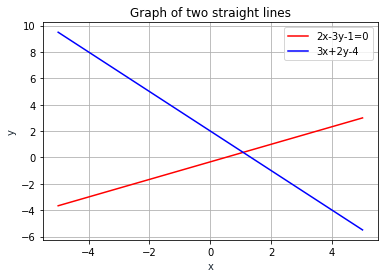
\includegraphics[width=\columnwidth]{A6.png}
    \caption{Pair of straight lines}
    \label{Fig :1}
\end{figure}
Python Code 
\begin{lstlisting}
https://github.com/ayushkesh/Matrix-Theory-EE5609/blob/master/A6/A6.ipynb
\end{lstlisting}
\end{document}
